\documentclass{article}
\usepackage[utf8]{inputenc}
\usepackage{fancyvrb}
\usepackage{hyperref}
\usepackage{graphicx}
\title{File/Data Formats in WifEye}
\author{Philipp H. Kindt, philipp.kindt@informatik.tu-chemnitz.de}
\begin{document}
\maketitle
	\section{Overview}
WifEye provides the following 3 different file formats for exporting CSI data:
\begin{itemize}
	\item \textbf{Simple CSV Format}: A comma-separated value (CSV) format optimized for simplicity. It is the only format used for live-export (e.g., streaming data to an external program such as a classifier in real-time). It can also be used for recording data to files.
	\item \textbf{Compact CSV Format}: A CSV format which demands only approximately 30\% of the space of the \textit{simple CSV} format. It can be used for recording data into files.
	\item \textbf{WifEye Binary:} A non-standard, proprietary file format with minimalistic space requirements. It requires less than about 20\% of the space of the \textit{Simple CSV} format and only 60\% of the space of the \textit{Compact CSV} format. It can be used for recording data into files. 
\end{itemize}
In addition, there is a dedicated exchange format to read classification results from a classifier into WifEye for the purpose of real-time annotations. Figure~\ref{fig:formatOverview} gives an overview on the different formats used in different data paths. This document describes all of these formats.
\begin{figure}
	\centering
	\vspace*{-.5cm}
	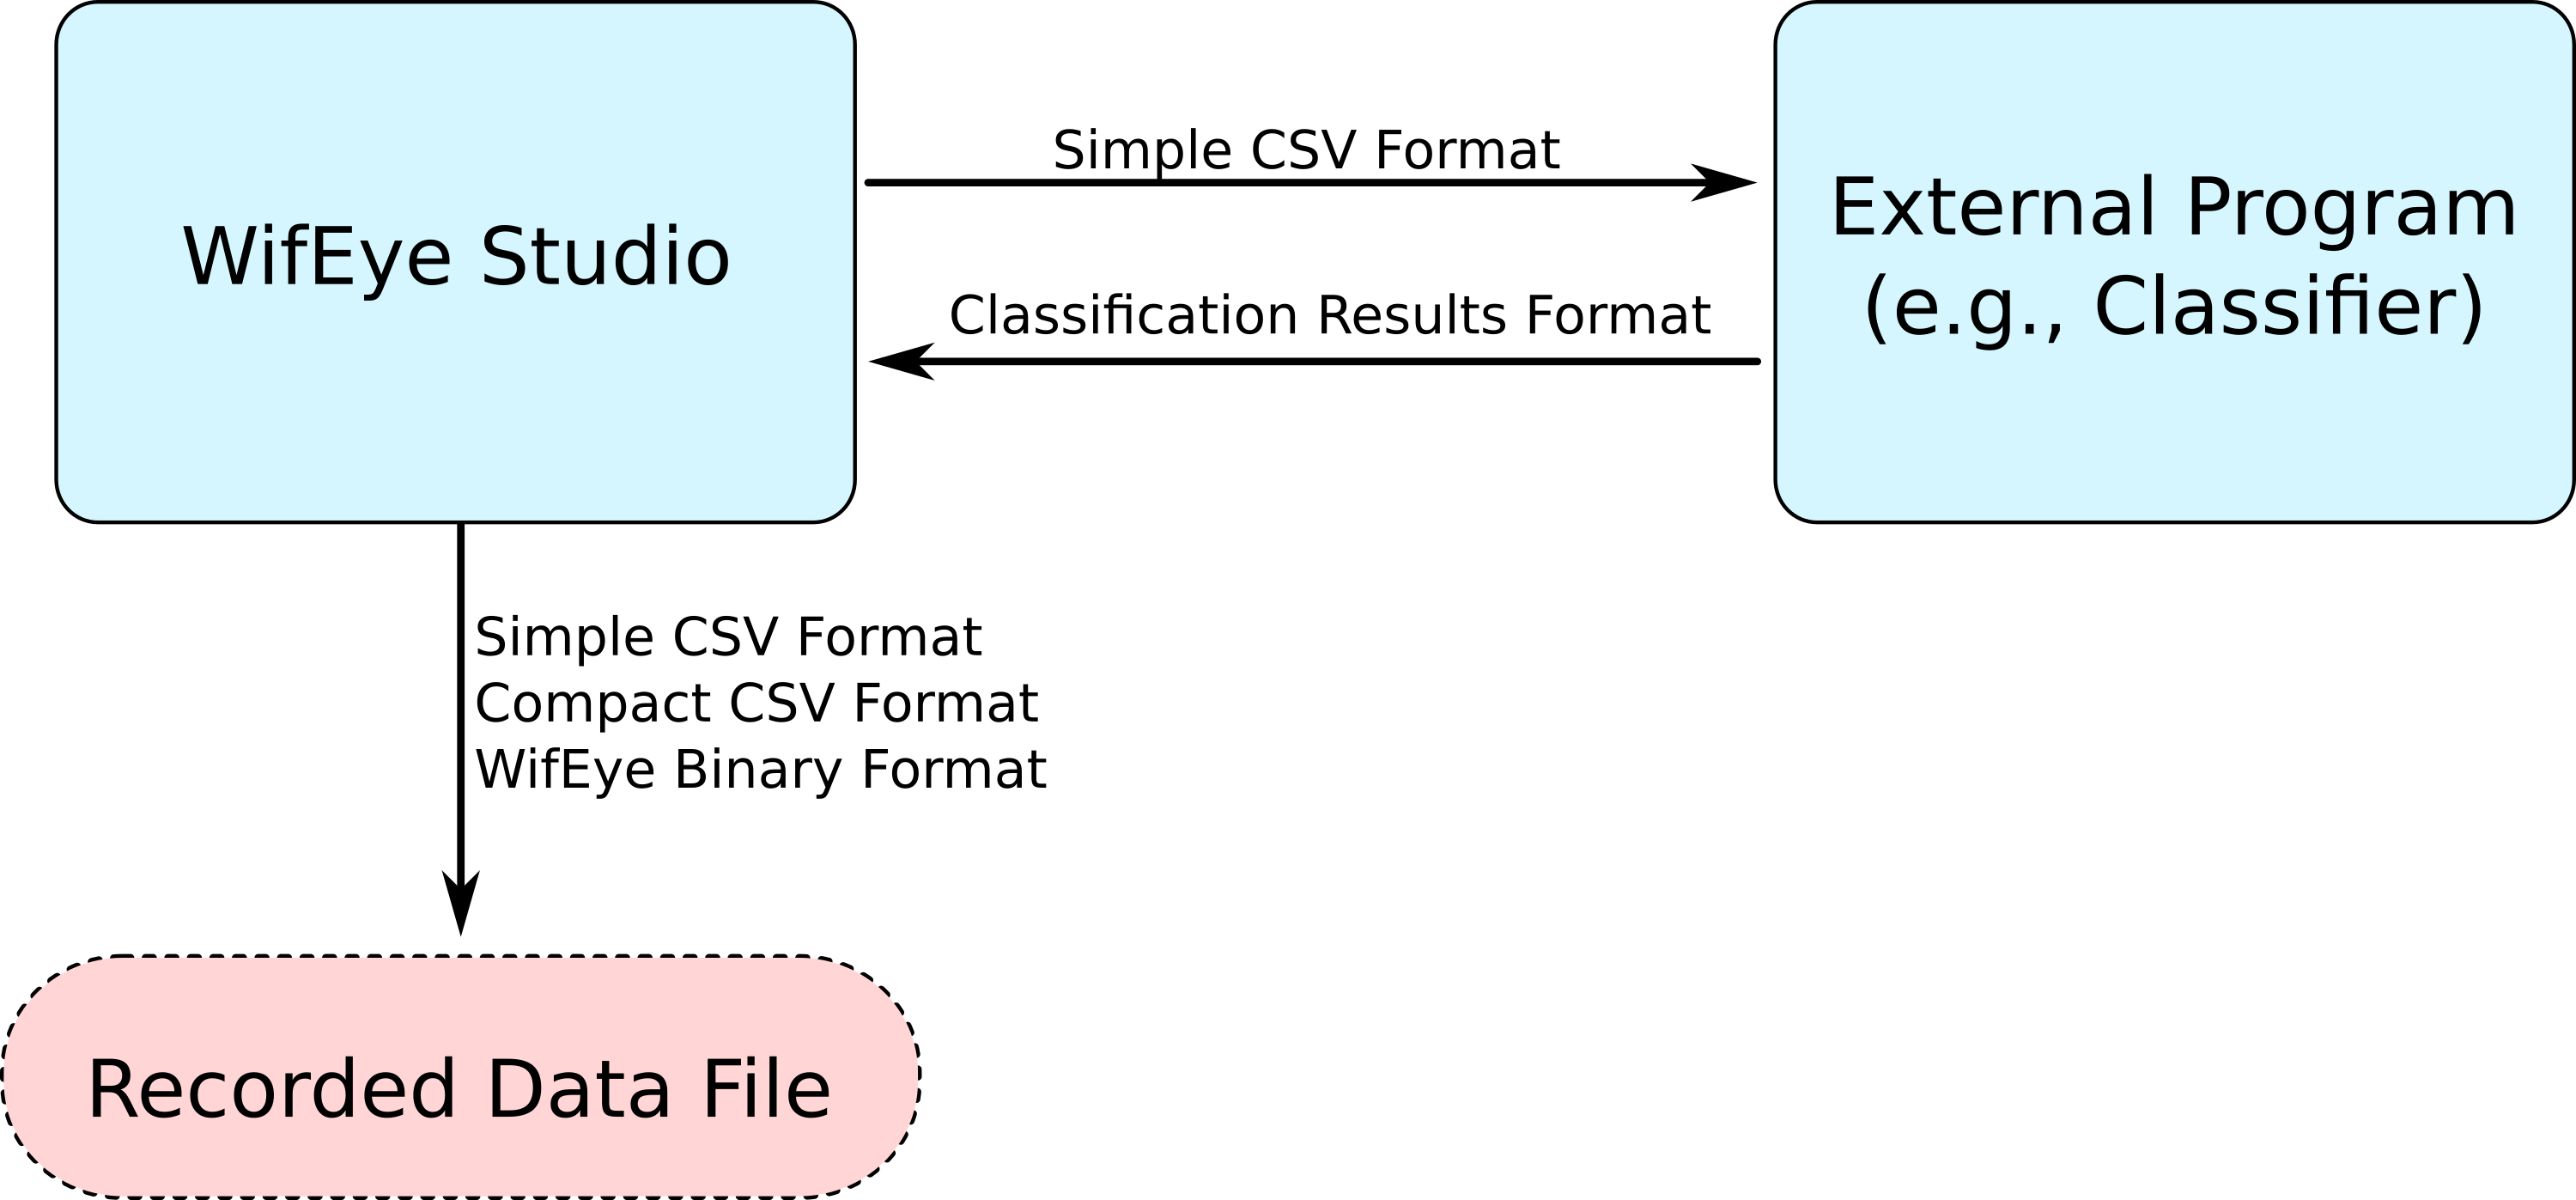
\includegraphics[width=0.8\textwidth]{images/formatOverview.png}
	\caption{Overview of the formats used.}
	\label{fig:formatOverview}
\end{figure}
\section{Simple CSV Format}
The \textit{simple CSV} format uses one line per subcarrier. Data of multiple subcarriers that belong to the same frame always appear subsequently (i.e., without any data belonging to a different frame in between), in ascending order by their subcarrier index. The disadvantage of this format is that data remaining the same for each subcarrier (e.g., the timestamp and the MAC address) is repeated for every single subcarrier, thereby occupying a considerable amount of additional space.

This format is used both for live-export to an external program, as well as for data-recording. The format is identical for both purposes, barring the only exception that for live-export, no CSV header is generated.
The CSV-header (which is used for recording data into files) is as follows.
\begin{Verbatim}[fontsize=\small]
timestamp;MAC;subcarrier;amplitude;phase;RSSI;frame_control
\end{Verbatim}
Each line of CSV data, which belongs to a single subcarrier, consists of the following data (in this order), each separated by a semicolon (``;'').
\begin{enumerate}
	\item The timestamp as a string ``yyyy-mm-dd hh-:ii:ss:uuuuuu)''. \textit{y} represents the year, \textit{m} the month, \textit{d} the day, \textit{h} the hour, \textit{i} the minute, \textit{s} the second and \textit{uu} the microseconds.
	\item The MAC address of the sender as a string with hexadecimal numbers. Each two characters are separated by a colon. E.g.,``ca:ff:ee:ca:ff:ee''.
	\item The subcarrier index as a counting number.
	\item The CSI amplitude as a floating point number. The decimal separator is always a dot (``.''), there are 10 digits behind the dot. Make sure that the \textit{en\_US} locale is installed before recording to ensure the right decimal separator is used.
	\item The CSI phase as a floating point number. The decimal separator is a dot (``.''), there are 10 digits behind the dot.
	\item The RSSI of the frame as a floating point number. The decimal separator is always a dot (``.'').
	\item The \textit{frame control} field as an integer between 0 and 255. 
\end{enumerate}
Example file (truncated after 10 rows of CSI data):
\begin{Verbatim}[fontsize=\small]
timestamp;MAC;subcarrier;amplitude;phase;RSSI;frame_control
2021-10-29 18:07:33:885002;34:31:c4:68:33:ba;0;0.0000000000;0,0000000000;-16.3306273036;128
2021-10-29 18:07:33:885002;34:31:c4:68:33:ba;1;0.0000000000;0,0000000000;-16.3306273036;128
2021-10-29 18:07:33:885002;34:31:c4:68:33:ba;2;0.0000000000;0,0000000000;-16.3306273036;128
2021-10-29 18:07:33:885002;34:31:c4:68:33:ba;3;0.0000000000;0,0000000000;-16.3306273036;128
2021-10-29 18:07:33:885002;34:31:c4:68:33:ba;4;0.0821877068;0,0000000000;-16.3306273036;128
2021-10-29 18:07:33:885002;34:31:c4:68:33:ba;5;0.0713229456;-1,7858112085;-16.3306273036;128
2021-10-29 18:07:33:885002;34:31:c4:68:33:ba;6;0.0376520662;-4.1719695729;-16.3306273036;128
2021-10-29 18:07:33:885002;34:31:c4:68:33:ba;7;0.0408393998;-4.1932428661;-16.3306273036;128
2021-10-29 18:07:33:885002;34:31:c4:68:33:ba;8;0.0091319674;-8.5526415515;-16.3306273036;128
2021-10-29 18:07:33:885002;34:31:c4:68:33:ba;9;0.0547918045;-9.1277138412;-16.3306273036;128
\end{Verbatim}

\section{Compact CSV Format}
A more compact data format, which can be used for recording data into files, is obtained by writing one line per frame (and not per subcarrier, as in the \textit{simple CSI} format).
The CSV header depends on the number of subcarriers (and hence on the channel bandwidth). For the most simple case of a 20 MHz channel that has 64 subcarriers, it looks as follows.
\begin{Verbatim}[fontsize=\small]
timestamp;MAC;RSSI;frame_control;a0;p0;a1;p1;a2;p2;a3;p3;a4;p4;a5;p5;a6;p6;a7;p7;a8;p8;a9;p9;
a10;p10;a11;p11;a12;p12;a13;p13;a14;p14;a15;p15;a16;p16;a17;p17;a18;p18;a19;p19;a20;p20;a21;
p21;a22;p22;a23;p23;a24;p24;a25;p25;a26;p26;a27;p27;a28;p28;a29;p29;a30;p30;a31;p31;a32;p32;
a33;p33;a34;p34;a35;p35;a36;p36;a37;p37;a38;p38;a39;p39;a40;p40;a41;p41;a42;p42;a43;p43;a44;
p44;a45;p45;a46;p46;a47;p47;a48;p48;a49;p49;a50;p50;a51;p51;a52;p52;a53;p53;a54;p54;a55;p55;
a56;p56;a57;p57;a58;p58;a59;p59;a60;p60;a61;p61;a62;p62;a63;p63
\end{Verbatim}
(note that there are no linebreaks in the CSV header).

Here, \textit{axy} represents the amplitude of subcarrier \textit{xy}. Similarly, \textit{pxy} corresponds to the phase of subcarrier \textit{xy}. The highest value of \textit{xy} and hence the header length depends on the 
number of subcarriers.
Every line contains the following data (in this order, separated by semicolons):
\begin{enumerate}
	\item The timestamp as a string ``yyyy-mm-dd hh-:ii:ss:uuuuuu)''. \textit{y} represents the year, \textit{m} the month, \textit{d} the day, \textit{h} the hour, \textit{i} the minute, \textit{s} the second and \textit{uu} the microseconds.
	\item The MAC address of the sender in hexadecimal format. Each two chars are separated by a colon. E.g.,``ca:ff:ee:ca:ff:ee''.
	\item The RSSI of the frame as a floating point number. The decimal separator is a dot (``.'').
	\item The \textit{frame control} field as an integer between 0 and 255.
	\item As many pairs of values of CSI amplitudes and phases as there are subcarriers.  Each amplitude or phase is represented by a floating point number. The decimal separator is a dot (``.''), there are 10 digits behind the dot.
\end{enumerate}
An example is omitted, since already one line of data would require excessive space in this document. You obtain an example by capturing a few frames using WifEye. The format is actually fully explained by the header.

\section{WifEye Binary (.wbin) Format}
The \textit{WifEye binary} format can be used for recording CSI data. Different from the other formats, the file ending is \textit{.wbin} instead of \textit{.csv}.
It is structured as follows.
\begin{enumerate}
	\item (12 Bytes) File header, consisting of the string ``WiFeyeBinary''.
	\item (4 Bytes) The number of subcarriers as a 32-bit unsigned integer.
	\item For every received frame:
	\begin{enumerate}
		\item (16 bytes) A timestamp in format \textit{struct timespec\_16bytes} (see below). It is identical to \textit{struct timespec}, but always has 16 bytes of size, while the size of \textit{struct timespec} might be platform dependant. (16 bytes)
		\item (6 bytes) The MAC address.
		\item (8 bytes) The RSSI as a double precision floating point value.
		\item (1 byte) The frame-control field, which is usually interpreted as an unsigned integer.
		\item For each subcarrier of the frame:
		\begin{enumerate}
			\item (8 bytes) The CSI amplitude of that subcarrier as a double precision floating point value.
			\item (8 bytes) The CSI phase of that subcarrier as a double precision floating point value.
		\end{enumerate}
	\end{enumerate}
\end{enumerate}
Below is a definition of \textit{struct timespec\_16bytes}:
\begin{verbatim}
struct timespec_16bytes{
	uint64_t tv_sec;
	uint64_t tv_nsec;
};
\end{verbatim}
Figure~\ref{fig:wbinformat} provides an example of the WifEye binary format.
A C-program to read this data can be found under the name \textit{readBinaryFormat.c} in the \textit{tools} folder of the WifEye repository.
\begin{figure}
\centering
\vspace*{-.5cm}
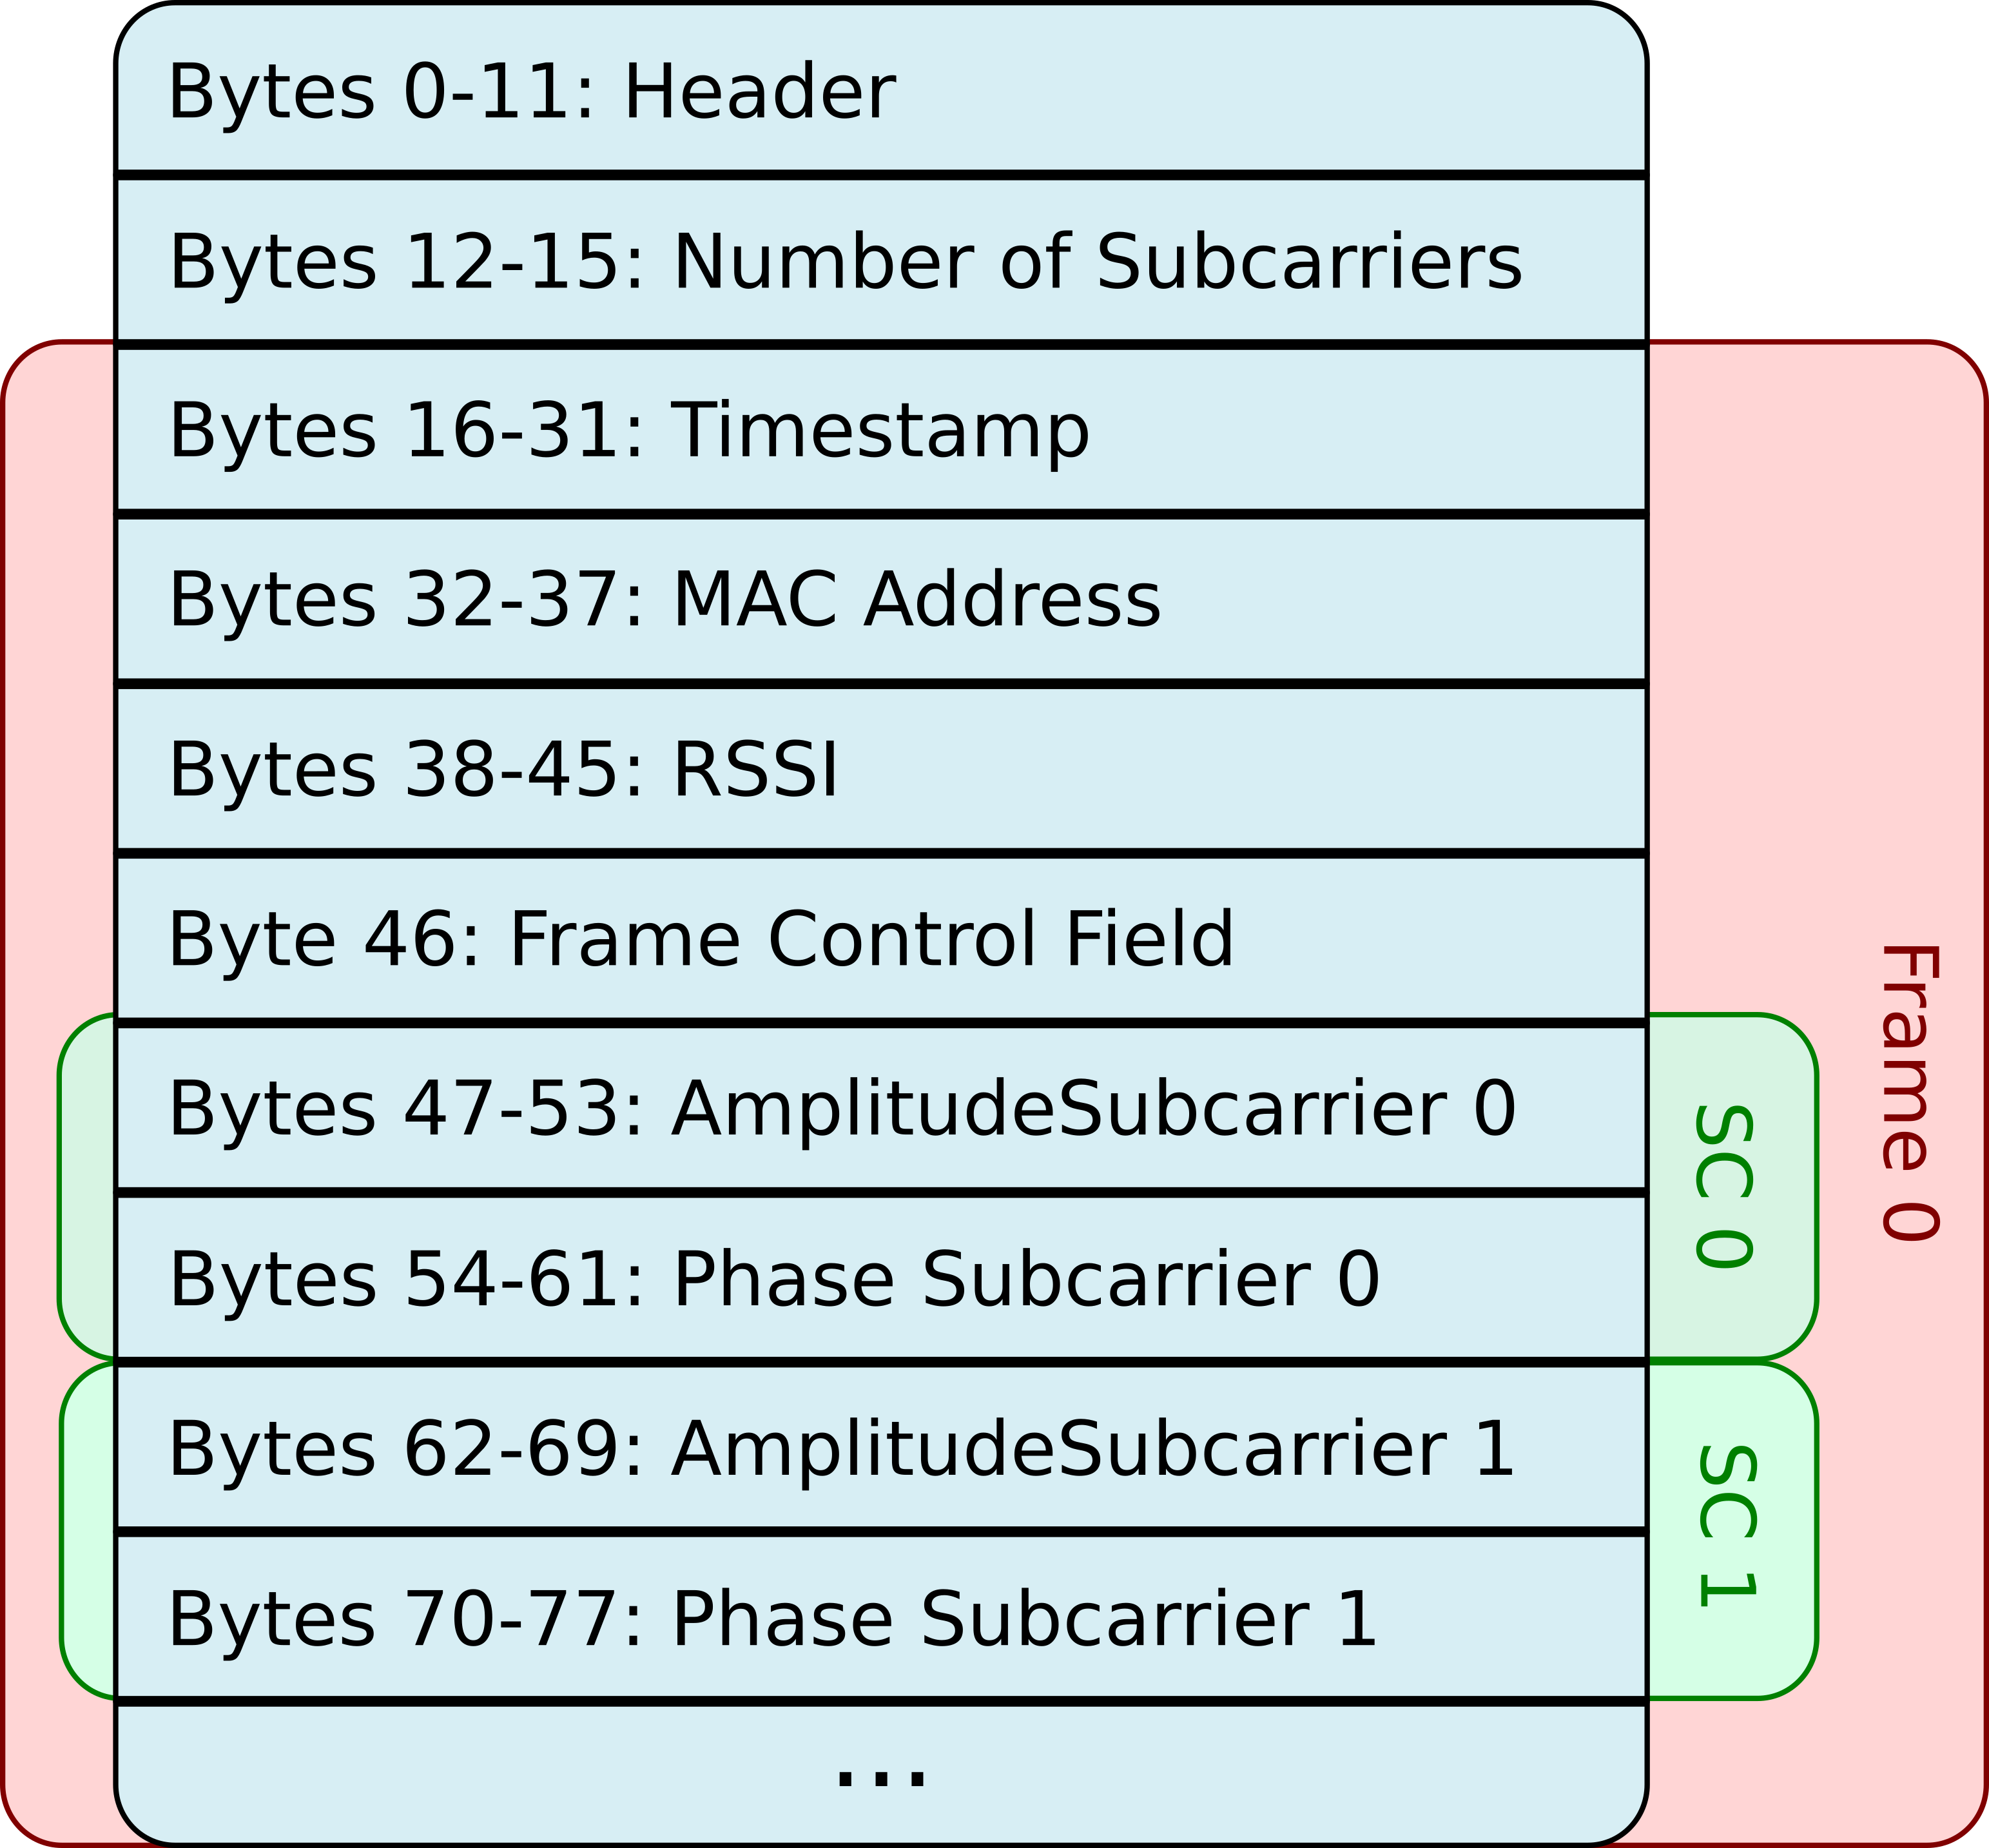
\includegraphics[width=0.5\textwidth]{images/wbinformat.png}
\caption{Example of the Wifeye Binary (\textit{.wbin}) format.}
\label{fig:wbinformat}
\end{figure}

\section{Data Format for Classification Results}
The format for signaling classification results consists of pairs of the class number to which the most recent data has been assigned to, and a confidence value. Each such pair belongs to a certain classifier - the number of classifiers can be arbitrarily high. Each value is separated by a semicolon (``:'') as follows:
\begin{verbatim}
class0:confidence0:class1:confidence1:class2:confidence2,...
\end{verbatim}
Here, the numbers ($0,1,2,...)$ identify the classifier. 
The class number is an integer and the highest possible class number needs to be defined in the settings of WifEye studio. The \textit{confidence} is a floating point value between $0$ (the classifier is not at all confident in the results) and $1$ (the classifier is 100 \% confident in the results). Each such classifier output is terminated by a newline. WifEye assumes that a classifier output belongs to all data since the previous output was received.
Example:
\begin{verbatim}
5:0.01:9:0.99
\end{verbatim}
Note that each line must contain an output of \emph{all} classifiers. If some classifiers have not yet computed a new result, the previous result needs to be repeated in such cases. 
\end{document}
